\documentclass[12pt,a4paper]{article}
\usepackage[top=2.5cm,bottom=2.5cm,left=2.5cm,right=2.5cm,headheight=15pt]{geometry}
\usepackage{amsmath,amssymb}
\usepackage{tikz}
\usetikzlibrary{shapes,arrows,arrows.meta,positioning,calc,backgrounds,fit,matrix}
\usepackage{booktabs,array,longtable,tabularx,multirow}
\usepackage{xcolor}
\usepackage{enumitem}
\usepackage{fancyhdr}
\usepackage{titlesec}
\usepackage{mdframed}
\usepackage{tcolorbox}
\tcbuselibrary{skins,breakable}
\usepackage{hyperref}

%% ---- Colors ----
\definecolor{folblue}{RGB}{0,82,165}
\definecolor{lightblue}{RGB}{220,235,255}
\definecolor{darkorange}{RGB}{180,70,0}
\definecolor{lightorange}{RGB}{255,235,210}
\definecolor{darkgreen}{RGB}{20,110,20}
\definecolor{lightgreen}{RGB}{200,240,205}
\definecolor{darkred}{RGB}{150,20,20}
\definecolor{lightred}{RGB}{255,210,210}
\definecolor{lightgray}{RGB}{242,242,242}

%% ---- tcolorbox styles ----
\newtcolorbox{qbox}[2][]{enhanced,breakable,
  colback=lightorange,colframe=darkorange,arc=4pt,
  title={\textbf{#2}},fonttitle=\bfseries\color{white},
  attach boxed title to top left={yshift=-2mm,xshift=4mm},
  boxed title style={colback=darkorange,arc=3pt},#1}

\newtcolorbox{solbox}[2][]{enhanced,breakable,
  colback=lightblue,colframe=folblue,arc=4pt,
  title={\textbf{#2}},fonttitle=\bfseries\color{white},
  attach boxed title to top left={yshift=-2mm,xshift=4mm},
  boxed title style={colback=folblue,arc=3pt},#1}

\newtcolorbox{keybox}[2][]{enhanced,breakable,
  colback=lightgreen,colframe=darkgreen,arc=4pt,
  title={\textbf{#2}},fonttitle=\bfseries\color{white},
  attach boxed title to top left={yshift=-2mm,xshift=4mm},
  boxed title style={colback=darkgreen,arc=3pt},#1}

\newtcolorbox{algobox}[2][]{enhanced,breakable,
  colback=lightgray,colframe=gray!60,arc=4pt,
  title={\textbf{#2}},fonttitle=\bfseries,
  attach boxed title to top left={yshift=-2mm,xshift=4mm},
  boxed title style={colback=gray!60,arc=3pt},#1}

\newtcolorbox{warnbox}[2][]{enhanced,breakable,
  colback=lightred,colframe=darkred,arc=4pt,
  title={\textbf{#2}},fonttitle=\bfseries\color{white},
  attach boxed title to top left={yshift=-2mm,xshift=4mm},
  boxed title style={colback=darkred,arc=3pt},#1}

%% ---- Page style ----
\pagestyle{fancy}\fancyhf{}
\lhead{\color{folblue}\textbf{AES --- CSE 717 InfoSec}}
\rhead{\color{folblue}Exam: 17 Jun 2026}
\cfoot{--- \thepage\ ---}
\renewcommand{\headrulewidth}{0.4pt}

%% ---- Section style ----
\titleformat{\section}{\large\bfseries\color{folblue}}{}{0em}{}[\titlerule]
\titleformat{\subsection}{\normalsize\bfseries\color{darkorange}}{}{0em}{}

\begin{document}

\begin{center}
{\LARGE\bfseries\color{folblue} CSE 717 --- Information Security}\\[4pt]
{\large\bfseries Topic 9: AES --- S-box (GF(2$^8$)), ShiftRows, MixColumns, Block Diagram}\\[2pt]
{\large Complete Past Paper Solutions: 2020--2024}\\[6pt]
{\normalsize Source: Lc\#8 pp2--13 (AES Algorithm in Cryptography)}\\[2pt]
{\normalsize\color{darkred}\textbf{4/5 years, 4--6 marks. Block diagram is a near-certain ``draw it'' question (2021, 2023, 2024).}}
\end{center}

\tableofcontents

%% ==========================================
\section*{Quick Reference --- The AES Round (CHEAT SHEET)}
%% ==========================================

\begin{warnbox}{What AES actually is}
AES encrypts a \textbf{128-bit block} (16 bytes) arranged as a $4\times4$ \textbf{state matrix}, filled \textbf{column by column}. Key size determines the number of rounds: \textbf{10 rounds for 128-bit keys}, 12 for 192-bit, 14 for 256-bit. (Lc\#8 p5 --- exam always uses 128-bit/10-round AES.)
\end{warnbox}

\begin{algobox}{Plaintext $\to$ State Matrix (Lc\#8 p3)}
Convert each character to its ASCII hex code, then fill the $4\times4$ matrix \textbf{column-major} (top-to-bottom, then next column). If the plaintext is shorter than 16 bytes, pad (slide example pads with `Z'=19 hex).

\textbf{Example:} ``AES USES A MATRIX'' $\to$ hex stream \texttt{00 04 12 14 12 04 12 00 0C 00 13 11 08 17 19 19} $\to$
\[
\text{State}=
\begin{bmatrix}
00 & 12 & 0C & 08\\
04 & 04 & 00 & 17\\
12 & 12 & 13 & 19\\
14 & 00 & 11 & 19
\end{bmatrix}
\]
(column 0 = first 4 bytes, column 1 = next 4 bytes, etc.)
\end{algobox}

\begin{algobox}{AES-128 Encryption Structure --- 10 Rounds (Lc\#8 p5)}
\begin{enumerate}[noitemsep]
  \item \textbf{Initial step:} AddRoundKey with $K_0$.
  \item \textbf{Rounds 1--9 (each identical):} SubBytes $\to$ ShiftRows $\to$ MixColumns $\to$ AddRoundKey($K_i$).
  \item \textbf{Round 10 (final, different):} SubBytes $\to$ ShiftRows $\to$ AddRoundKey($K_{10}$) --- \textbf{no MixColumns}.
\end{enumerate}
\textit{This 9$\times$(4 steps) + 1$\times$(3 steps) + 1 initial AddRoundKey is exactly what the block diagram (2021/2023/2024) must show.}
\end{algobox}

\begin{keybox}{The 4 round operations --- one-line definitions}
\begin{itemize}[noitemsep]
  \item \textbf{SubBytes:} replace each byte with its S-box value. Split byte into (row, col) hex nibbles, look up table. \textit{Example: EA $\to$ 87} (row E, col A).
  \item \textbf{ShiftRows:} cyclic LEFT shift of each row of the state matrix --- Row 0: no shift; Row 1: shift left 1; Row 2: shift left 2; Row 3: shift left 3 (Lc\#8 p7).
  \item \textbf{MixColumns:} multiply each column by the fixed matrix $\begin{bmatrix}02&03&01&01\\01&02&03&01\\01&01&02&03\\03&01&01&02\end{bmatrix}$ in GF($2^8$), XOR-ing the products.
  \item \textbf{AddRoundKey:} bitwise XOR the state matrix with the round-key matrix.
\end{itemize}
\end{keybox}

\begin{keybox}{GF($2^8$) multiplication rules for MixColumns (Lc\#8 p10)}
\begin{itemize}[noitemsep]
  \item $01 \times x = x$ (identity).
  \item $02 \times x$ = left-shift $x$ by 1 bit; if the bit shifted out (MSB) was 1, XOR the result with \texttt{1B}.
  \item $03 \times x = (02\times x)\oplus x$.
  \item Higher multipliers: $04\times x = 02\times(02\times x)$, $08\times x=02\times(04\times x)$, etc. (repeated doubling).
  \item All bytes represent polynomials of degree $\le 7$ --- results always stay one byte (8 bits).
\end{itemize}
\end{keybox}

%% ==========================================
\section{AES Encryption Block Diagram (recurring: 2021 B1(a) 4.75, 2023 Q3(c) 4, 2024 Q3(c) 2)}
%% ==========================================

\begin{qbox}{Question --- 2021 Section B Q1(a) [4.75], 2023 Q3(c) [4], 2024 Q3(c) [2]}
Draw and explain the AES encryption block diagram, showing all rounds and the operations performed in each round.
\end{qbox}

\begin{solbox}{Answer --- the diagram (memorize this exact structure)}
\begin{center}
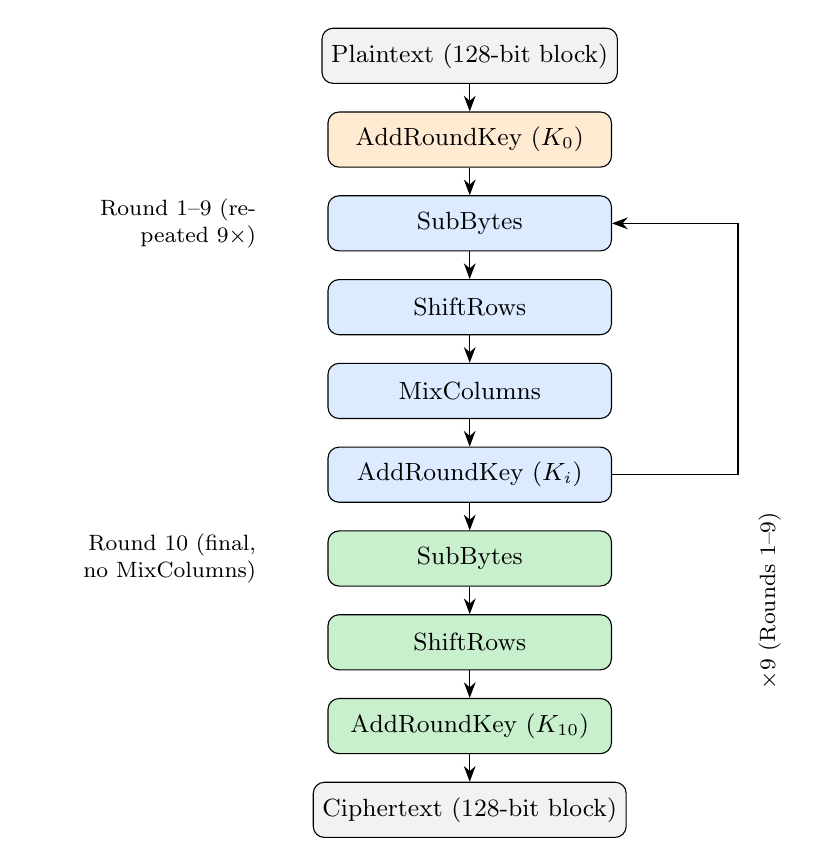
\begin{tikzpicture}[
  every node/.style={font=\small, draw, rounded corners, minimum width=3.6cm, minimum height=0.7cm, align=center},
  node distance=0.35cm
]
\node[fill=lightgray] (pt) {Plaintext (128-bit block)};
\node[fill=lightorange, below=of pt] (ark0) {AddRoundKey ($K_0$)};
\node[fill=lightblue, below=of ark0] (sb) {SubBytes};
\node[fill=lightblue, below=of sb] (sr) {ShiftRows};
\node[fill=lightblue, below=of sr] (mc) {MixColumns};
\node[fill=lightblue, below=of mc] (arki) {AddRoundKey ($K_i$)};
\node[fill=lightgreen, below=of arki] (sb2) {SubBytes};
\node[fill=lightgreen, below=of sb2] (sr2) {ShiftRows};
\node[fill=lightgreen, below=of sr2] (ark10) {AddRoundKey ($K_{10}$)};
\node[fill=lightgray, below=of ark10] (ct) {Ciphertext (128-bit block)};

\draw[-{Stealth[length=2mm]}] (pt) -- (ark0);
\draw[-{Stealth[length=2mm]}] (ark0) -- (sb);
\draw[-{Stealth[length=2mm]}] (sb) -- (sr);
\draw[-{Stealth[length=2mm]}] (sr) -- (mc);
\draw[-{Stealth[length=2mm]}] (mc) -- (arki);
\draw[-{Stealth[length=2mm]}] (arki) -- (sb2);
\draw[-{Stealth[length=2mm]}] (sb2) -- (sr2);
\draw[-{Stealth[length=2mm]}] (sr2) -- (ark10);
\draw[-{Stealth[length=2mm]}] (ark10) -- (ct);

% loop arrow for rounds 1-9
\draw[-{Stealth[length=2mm]}] (arki.east) -- ++(1.6,0) |- (sb.east);
\node[draw=none, fill=none, rotate=90, anchor=center] at ($(arki.east)+(2.0,-1.6)$) {\footnotesize $\times 9$ (Rounds 1--9)};

\node[draw=none, fill=none, left=0.2cm of sb, font=\footnotesize, align=right, text width=2.2cm] {Round 1--9 (repeated 9$\times$)};
\node[draw=none, fill=none, left=0.2cm of sb2, font=\footnotesize, align=right, text width=2.2cm] {Round 10 (final, no MixColumns)};
\end{tikzpicture}
\end{center}

\textbf{Explanation to write alongside the diagram:}
\begin{itemize}[noitemsep]
  \item AES-128 uses \textbf{10 rounds}. Before round 1, the plaintext state is XOR'd with the initial round key $K_0$ (\textbf{AddRoundKey}).
  \item \textbf{Rounds 1--9} are identical: \textbf{SubBytes} (non-linear byte substitution via S-box) $\to$ \textbf{ShiftRows} (cyclic row shifts $\to$ diffusion across columns) $\to$ \textbf{MixColumns} (linear mixing within each column over GF($2^8$) $\to$ diffusion within columns) $\to$ \textbf{AddRoundKey} (XOR with that round's subkey $K_i$, derived via key expansion).
  \item \textbf{Round 10 (final round)} drops MixColumns: SubBytes $\to$ ShiftRows $\to$ AddRoundKey($K_{10}$) only --- this makes encryption and decryption structurally invertible.
  \item Output of round 10 = \textbf{ciphertext} (128-bit block).
\end{itemize}
\end{solbox}

%% ==========================================
\section{2024 --- Q3(a): ShiftRows+MixColumns diffusion (4); Q3(c): block diagram (2)}
%% ==========================================

\begin{qbox}{Question --- 2024 Q3(a)\&(c)}
\begin{enumerate}[label=(\alph*)]
  \item[(a)] Explain how ShiftRows and MixColumns provide diffusion in AES. Given the state matrix below, perform the ShiftRows operation and show the result. \hfill [4]
\[
\text{State}=
\begin{bmatrix}
\texttt{d4} & \texttt{e0} & \texttt{b8} & \texttt{1e}\\
\texttt{27} & \texttt{bf} & \texttt{b4} & \texttt{41}\\
\texttt{11} & \texttt{98} & \texttt{5d} & \texttt{52}\\
\texttt{ae} & \texttt{f1} & \texttt{e5} & \texttt{30}
\end{bmatrix}
\]
  \item[(c)] Draw the AES encryption block diagram. \hfill [2]
\end{enumerate}
\end{qbox}

\subsection{Part (a): Diffusion explanation + ShiftRows trace}
\begin{solbox}{Answer --- 2024 Q3(a)}
\textbf{How ShiftRows provides diffusion:} each row of the state is cyclically shifted left by a different amount (0,1,2,3 bytes). This moves bytes \textbf{between columns}, so after MixColumns (which operates per-column), every output byte of a column depends on bytes that originally came from \textbf{four different columns} of the input. A single-byte change in the plaintext spreads across the entire state within a couple of rounds --- this spreading property is \textbf{diffusion}.

\textbf{How MixColumns provides diffusion:} it treats each column as a 4-byte vector and multiplies it by a fixed $4\times4$ matrix over GF($2^8$) (Lc\#8 p9-12). Every output byte in a column is a GF($2^8$) linear combination of \textbf{all 4 input bytes} of that column. Combined with ShiftRows (which mixes bytes across columns first), repeated rounds cause every output bit to depend on every input bit and every key bit --- the \textbf{avalanche effect}.

\textbf{ShiftRows trace on the given state} --- apply the rule (Row 0: no shift; Row 1: left-shift 1; Row 2: left-shift 2; Row 3: left-shift 3):

\renewcommand{\arraystretch}{1.2}
\begin{center}
\begin{tabular}{lcccc}
\toprule
Row & Before & Shift & \multicolumn{2}{c}{After} \\
\midrule
0 & \texttt{d4 e0 b8 1e} & none & \multicolumn{2}{c}{\texttt{d4 e0 b8 1e}} \\
1 & \texttt{27 bf b4 41} & left 1 & \multicolumn{2}{c}{\texttt{bf b4 41 27}} \\
2 & \texttt{11 98 5d 52} & left 2 & \multicolumn{2}{c}{\texttt{5d 52 11 98}} \\
3 & \texttt{ae f1 e5 30} & left 3 & \multicolumn{2}{c}{\texttt{30 ae f1 e5}} \\
\bottomrule
\end{tabular}
\end{center}

\[
\text{Result}=
\begin{bmatrix}
\texttt{d4} & \texttt{e0} & \texttt{b8} & \texttt{1e}\\
\texttt{bf} & \texttt{b4} & \texttt{41} & \texttt{27}\\
\texttt{5d} & \texttt{52} & \texttt{11} & \texttt{98}\\
\texttt{30} & \texttt{ae} & \texttt{f1} & \texttt{e5}
\end{bmatrix}
\]
\end{solbox}

\subsection{Part (c): Block diagram}
\begin{solbox}{Answer --- 2024 Q3(c)}
Same diagram as Section 1 above --- AddRoundKey($K_0$) $\to$ 9$\times$[SubBytes $\to$ ShiftRows $\to$ MixColumns $\to$ AddRoundKey] $\to$ [SubBytes $\to$ ShiftRows $\to$ AddRoundKey($K_{10}$)] $\to$ Ciphertext.
\end{solbox}

%% ==========================================
\section{2022 --- Section B Q5: S-box$(A_i)$ via GF($2^8$) multiplicative inverse (1.5+4.5)}
%% ==========================================

\begin{qbox}{Question --- 2022 Section B Q5}
Given $A_i = (11000010)_2$, find $A_i$ in hexadecimal. Using the GF($2^8$) multiplicative inverse table provided, compute $S(A_i)$, the AES S-box value of $A_i$. \hfill [1.5+4.5]
\end{qbox}

\begin{solbox}{Answer --- 2022 Section B Q5}
\textbf{Step 1 --- binary to hex:} $A_i=(11000010)_2 = \texttt{C2}_{16}$.

\textbf{Step 2 --- GF($2^8$) multiplicative inverse:} look up row \texttt{C}, column \texttt{2} in the multiplicative-inverse table (provided in the paper):
\[
\text{inv}(\texttt{C2}) = \texttt{2F}
\]

\textbf{Step 3 --- affine transformation:} the AES S-box is $S(x) = \text{Affine}(\text{inv}(x))$, where for $b=\text{inv}(x)$ with bits $b_7\ldots b_0$ ($b_0$ = LSB) and constant $c=\texttt{63}=01100011_2$:
\[
b'_i = b_i \oplus b_{(i+4)\bmod 8} \oplus b_{(i+5)\bmod 8} \oplus b_{(i+6)\bmod 8} \oplus b_{(i+7)\bmod 8} \oplus c_i
\]

$b=\texttt{2F}=00101111_2$ (so $b_7..b_0 = 0,0,1,0,1,1,1,1$), $c=01100011_2$ ($c_7..c_0=0,1,1,0,0,0,1,1$):

\renewcommand{\arraystretch}{1.15}
\begin{center}
\begin{tabular}{ccccccc}
\toprule
$i$ & $b_i$ & $b_{i+4}$ & $b_{i+5}$ & $b_{i+6}$ & $b_{i+7}$ & $c_i$ \quad$\Rightarrow b'_i$\\
\midrule
0 & 1 & 0 & 1 & 0 & 0 & 1 $\Rightarrow 1$\\
1 & 1 & 1 & 0 & 0 & 1 & 1 $\Rightarrow 0$\\
2 & 1 & 0 & 0 & 1 & 1 & 0 $\Rightarrow 1$\\
3 & 1 & 0 & 1 & 1 & 1 & 0 $\Rightarrow 0$\\
4 & 0 & 1 & 1 & 1 & 1 & 0 $\Rightarrow 0$\\
5 & 1 & 1 & 1 & 1 & 0 & 1 $\Rightarrow 0$\\
6 & 0 & 1 & 1 & 0 & 1 & 1 $\Rightarrow 0$\\
7 & 0 & 1 & 0 & 1 & 0 & 0 $\Rightarrow 0$\\
\bottomrule
\end{tabular}
\end{center}

(each $b'_i$ is the XOR of all six listed bits, all subscripts mod 8.)

\[
b' = b'_7b'_6b'_5b'_4b'_3b'_2b'_1b'_0 = 00100101_2 = \boxed{\texttt{25}}
\]

\[
\Rightarrow S(\texttt{C2}) = \boxed{\texttt{25}}
\]

\textit{Cross-check: this matches the AES S-box table (Lc\#8 p6) directly --- row \texttt{C}, column \texttt{2} of the S-box table also reads \texttt{25}. In the exam, if the S-box table is given directly (not the inverse table), skip Steps 2--3 and just look up the S-box table row/column.}
\end{solbox}

%% ==========================================
\section*{2020 --- No dedicated AES question found}
%% ==========================================
\begin{warnbox}{2020 paper}
No AES-specific question was identified in the 2020 past paper (Group A/B reviewed in full). AES coverage starts from 2021 onward. Do not over-invest extra prep specifically for a ``2020-style'' AES question --- focus on the recurring block-diagram + S-box + ShiftRows patterns above.
\end{warnbox}

%% ==========================================
\section*{Worked Reference --- MixColumns Full Example (Lc\#8 pp9--12)}
%% ==========================================

\begin{algobox}{MixColumns worked example from slides --- column $[\texttt{87},\texttt{6E},\texttt{46},\texttt{A6}]^T \to [\texttt{47},\ldots]^T$}
MixColumns formula for row 0 of a column: $s'_{0,j}=(02\cdot s_{0,j})\oplus(03\cdot s_{1,j})\oplus s_{2,j}\oplus s_{3,j}$.

Take column $[s_{0,j},s_{1,j},s_{2,j},s_{3,j}]=[\texttt{87},\texttt{6E},\texttt{46},\texttt{A6}]$:
\begin{itemize}[noitemsep]
  \item $02\times\texttt{87}$: $\texttt{87}=10000111_2$, left-shift $\to 00001110_2=\texttt{0E}$ (MSB was 1, so XOR \texttt{1B}): $\texttt{0E}\oplus\texttt{1B}=\texttt{15}$.
  \item $03\times\texttt{6E} = (02\times\texttt{6E})\oplus\texttt{6E}$: $\texttt{6E}<<1=\texttt{DC}$ (no overflow), $\texttt{DC}\oplus\texttt{6E}=\texttt{B2}$.
  \item $01\times\texttt{46}=\texttt{46}$, \quad $01\times\texttt{A6}=\texttt{A6}$.
  \item Sum: $\texttt{15}\oplus\texttt{B2}\oplus\texttt{46}\oplus\texttt{A6}$. Step by step: $\texttt{15}\oplus\texttt{B2}=\texttt{A7}$; $\texttt{A7}\oplus\texttt{46}=\texttt{E1}$; $\texttt{E1}\oplus\texttt{A6}=\boxed{\texttt{47}}$.
\end{itemize}
$\Rightarrow s'_{0,j}=\texttt{47}$ (the same procedure with the other 3 matrix rows gives the rest of the new column). The full new state's first column becomes $[\texttt{47},\texttt{37},\texttt{94},\texttt{ED}]^T$.

\textbf{AddRoundKey example (Lc\#8 p13):} $\texttt{47}\oplus\texttt{AC}$: $\texttt{47}=01000111_2$, $\texttt{AC}=10101100_2$, XOR $=11101011_2=\texttt{EB}$. Same byte-wise XOR is applied to the whole $4\times4$ state against the round-key matrix.
\end{algobox}

%% ==========================================
\section*{Exam Strategy Summary}
%% ==========================================

\begin{keybox}{High-Yield Checklist for AES (4/5 years, 4--6 marks)}
\begin{enumerate}[noitemsep]
  \item \textbf{Block diagram is near-guaranteed} (2021/23/24): memorize the 10-round structure --- AddRoundKey($K_0$), then 9$\times$[SubBytes$\to$ShiftRows$\to$MixColumns$\to$AddRoundKey], final round drops MixColumns.
  \item \textbf{ShiftRows:} Row 0 none, Row 1 left-1, Row 2 left-2, Row 3 left-3 --- cyclic LEFT shifts on state matrix rows (2024 Q3(a)).
  \item \textbf{S-box via GF($2^8$) inverse} (2022): hex split (row=high nibble, col=low nibble) $\to$ inverse table $\to$ affine transform with $c=\texttt{63}$; OR read S-box table directly if given.
  \item \textbf{MixColumns rules:} $01\times x=x$; $02\times x$=left-shift, XOR \texttt{1B} if overflow; $03\times x=(02\times x)\oplus x$. Practice one column by hand.
  \item \textbf{Diffusion} (2024): ShiftRows mixes across columns, MixColumns mixes within a column $\to$ avalanche effect.
  \item \textbf{Plaintext-to-state matrix} fill order is \textbf{column-major}.
\end{enumerate}
\end{keybox}

\end{document}
